\section{Jonathan}
\subsection{Overview}
\begin{frame}{Jonathan: Overview}
\begin{itemize}
\item GUI Requirements Analysis
\item REST Architecture Design
\item New Stuff?
\end{itemize}
\end{frame}

\subsection{GUI Requirements Analysis}
\begin{frame}{GUI Requirements Analysis}
A collaboration between SW609, SW610 and SW612.\\

A couple of the more noteworthy questions from the first meeting:
\begin{itemize}
\item How should switching from Guardian to Citizen and back happen?
\item Can there be multiple Guardians pr. Citizen?
\item Who are supposed to login?
\end{itemize}

\end{frame}

\begin{frame}[fragile]{GUI Requirements Analysis}
A couple of the more noteworthy requirements:

\begin{itemize}
\item There needs to be an option for grayscale.
\item If the system crashes it needs to return to a stable state or return to the Launcher
\item The QR-system needs to be replaced by a password based system.
\item Citizens should not be logged out automatically.
\item There should be an institute type user.
\end{itemize}
\end{frame}

\subsection{REST Architectural Design}
\begin{frame}{REST Architectural Design}
A Collaboration between SW609, SW610, SW613 and SW615.\\

The old client/server has serious problems, therefore make a new using the REpresentational State Transfer (REST) model which has the following requirements:
\begin{itemize}
\item Client-Server
\item Stateless
\item Cacheable
\item Layered System
\item Uniform Interface
\end{itemize}
\end{frame}

\begin{frame}{REST Architectural Design}
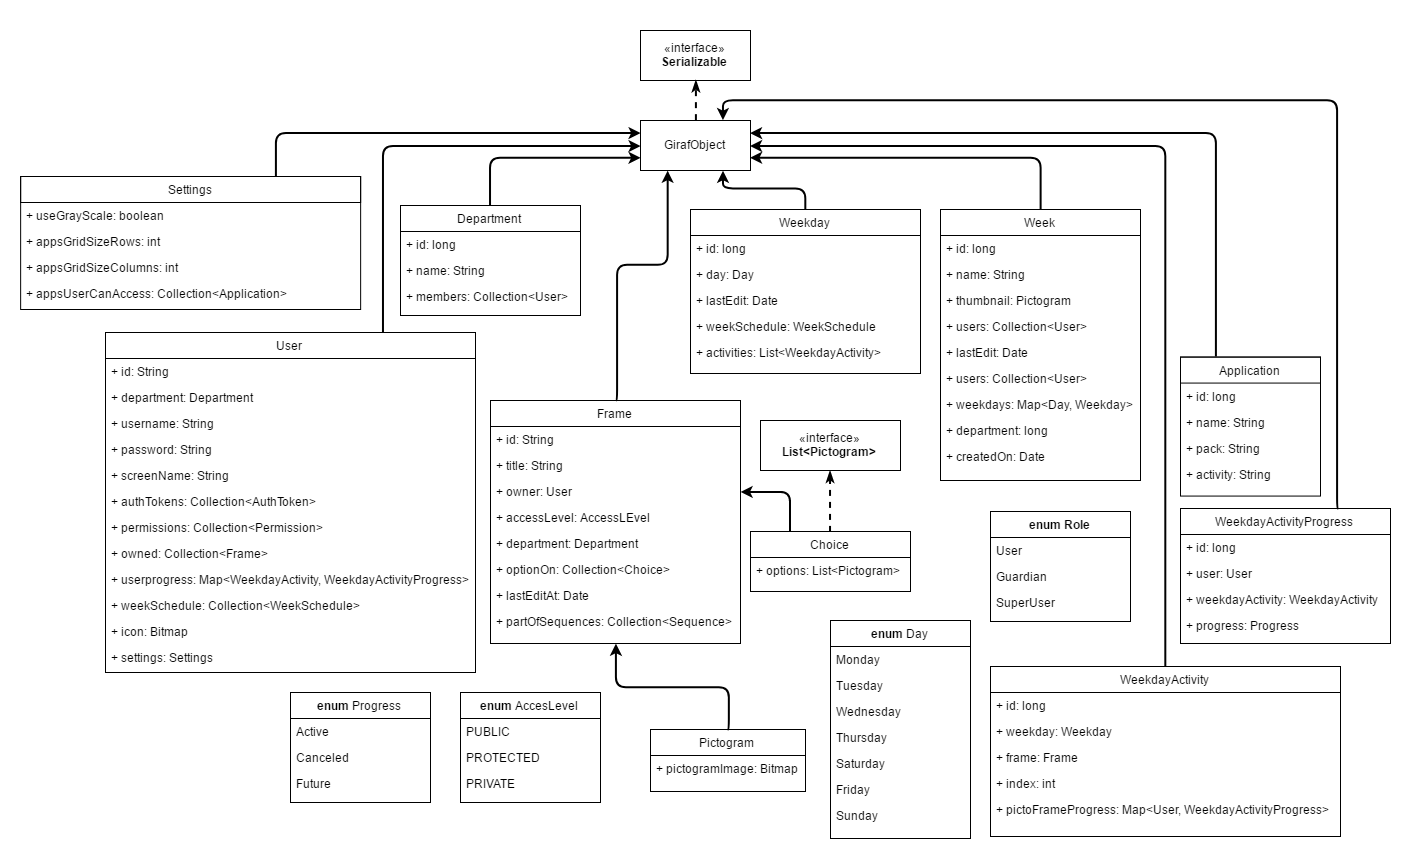
\includegraphics[scale=0.3]{figures/Giraf_RestModelV3.PNG}
\end{frame}

\begin{frame}{REST Architectural Design}

We use 3 different types of requests:
\begin{itemize}
\item LoginRequest
\item GetRequest
\item ResourceRequest
\end{itemize}

What is a Request and how do we use it?

\end{frame}

\begin{frame}[fragile]{REST Architectural Design}
Add a couple of example requests.

\begin{minipage}[H]{0.9\linewidth}
\begin{lstlisting}



\end{lstlisting}

\end{frame}

% \subsection{Network Structure}
% \begin{frame}{Network Structure}
% \begin{itemize}
% \item What does the network look like?
% \item Which features are used and how are their domains defined?
% \end{itemize}
% \begin{figure}
%   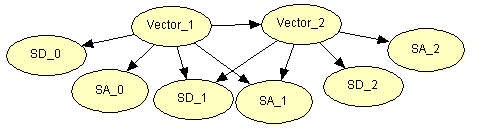
\includegraphics[scale=0.8]{figures/BNDone.PNG}
% \end{figure}
% \end{frame}
